%   MSc Business Analytics Dissertation
%   Format based on skeleton template provided as part of module MIS40750
%
%   Title:     Optimising the design of buffer preparation in bioprocessing
%              facilities
%   Author:    Sean Tully
%
%   Chapter 3: Data
%
%   Change Control:
%   When     Who   Ver  What
%   -------  ----  ---  --------------------------------------------------------
%   06Jun16  ST    0.1  Begun
%

\chapter{Data}\label{C.data}

\begin{quote}
We have some freedom in setting up our personal standards of beauty, but it is
especially nice when the things we regard as beautiful are also regarded by
other people as useful.

\hspace{2cm}--- Donald Knuth, \emph{Computer Programming as an Art}
\end{quote}

\section{Introduction}\label{S.intro3}
This chapter will outline the requirements for input data.

For modelling a single process, a typical data-set will consist of three
distinct files.
The first file is a table of data relating to the available selection of
vessels.
The second file is a table of data relating to parameters specific
to each buffer.
The third file comprises a collection of global parameters
that apply to all vessels and/or buffers.

One particular example, based on some randomly generated data, is used
throughout this chapter to illustrate the relevant data formats.

\section{Vessel Data}\label{S.vesseldata}

\begin{table}[h!]
    \centering
    \caption{Vessel data for random example}
    \label{tbl.vessel}
    \begin{tabular}{l | r | r}
        names & volumes & costs\\
        & $V_{m}$ (l) & $c_{m}$ (--)\\\hline
        \SI{1000}{\litre} & \SI{1000.0}{} & \SI{63.10}{}\\
        \SI{2000}{\litre} & \SI{2000.0}{} & \SI{95.64}{}\\
        \SI{3000}{\litre} & \SI{3000.0}{} & \SI{121.98}{}\\
        \SI{4000}{\litre} & \SI{4000.0}{} & \SI{144.96}{}\\
        \SI{5000}{\litre} & \SI{5000.0}{} & \SI{165.72}{}\\
        \SI{6000}{\litre} & \SI{6000.0}{} & \SI{184.88}{}\\
        \SI{8000}{\litre} & \SI{8000.0}{} & \SI{219.71}{}\\
        \SI{10000}{\litre} & \SI{10000.0}{} & \SI{251.19}{}\\
        \SI{12000}{\litre} & \SI{12000.0}{} & \SI{280.83}{}\\
        \SI{16000}{\litre} & \SI{16000.0}{} & \SI{333.02}{}\\
        \SI{18000}{\litre} & \SI{18000.0}{} & \SI{357.41}{}\\
        \SI{20000}{\litre} & \SI{20000.0}{} & \SI{380.73}{}\\
        \SI{22000}{\litre} & \SI{22000.0}{} & \SI{403.14}{}\\
        \SI{25000}{\litre} & \SI{25000.0}{} & \SI{435.28}{}\\
        \SI{30000}{\litre} & \SI{30000.0}{} & \SI{485.59}{}\\
    \end{tabular}
\end{table}

The vessel data will contain several parameters for each available vessel size,
$m \in \mathcal{M}$.
A vessel data-set will contain entries for $M$ vessel sizes:
\begin{equation}
    m \in \mathcal{M}; \quad \mathcal{M} = \left\{ 0, 1, 2, \ldots, m, \ldots,
    \left( M - 1 \right) \right\}
\end{equation}
\begin{equation}
    M = |\mathcal{M}|
\end{equation}

Note that the computer scientists' convention, whereby counting starts at zero,
is used throughout this report.

Typically, when designing a large-scale production facility, buffer preparation
vessel volumes range from \SI{1000}{\litre} to \SI{30000}{\litre}.

When ordering such a vessel, the stated size of the vessel is usually a nominal
volume, which may differ from the liquid fill volume and may also differ from
the maximum working volume.
It is usual to round the stated or nominal volume to the nearest thousand
litres.

For the purposes of this study, it is assumed that, for each vessel
$m \in \mathcal{M}$, the specified vessel volume, $V_{m}$, is the maximum
working volume (in litres) of the vessel. This is taken to be equivalent to
the maximum volume of buffer which can be prepared in that vessel.

Vessels will also have a minimum working volume.
It is usual to assume a minimum fill ratio of about 30\% of the vessel volume.
This limitation arises due to the minimum agitation volume of the impeller in
the vessel.
For the purposes of this simulation, the minimum fill ratio is a global
parameter.
It may be possible to specify a value of minimum fill ratio for every vessel
size, but this level of detail is typically neither required nor available.

For each vessel, $m \in \mathcal{M}$, a (relative) cost, $c_{m}$, must also be
defined.
Note that absolute costs are not required to find the vessel selection that
minimises costs.
Vessel costs tend not to scale linearly with volume.

Sample vessel data are given in \hyperref[tbl.vessel]{Table \ref*{tbl.vessel}}.
In this table, the cost value for each vessel size has been estimated by
raising the vessel volume (in litres) to a power of 0.6 and rounding to two
decimal places.
Note that the vessel volumes, $V_{m}$, are equal to the nominal volumes
indicated in the `names' column.  The contents of the `names' column are
treated as identifiers and are not used in any calculation.
It is not uncommon to have values of $V_{m}$ slightly larger than their
respective named (nominal) volumes; a vessel with a nominal volume of e.g.\
\SI{1000}{\litre} will be capable of holding at least \SI{1000}{\litre}, with
the precise maximum working volume being a function of the vessel geometry.

\section{Buffer Data}\label{S.bufferdata}
\begin{figure}
    \centering
    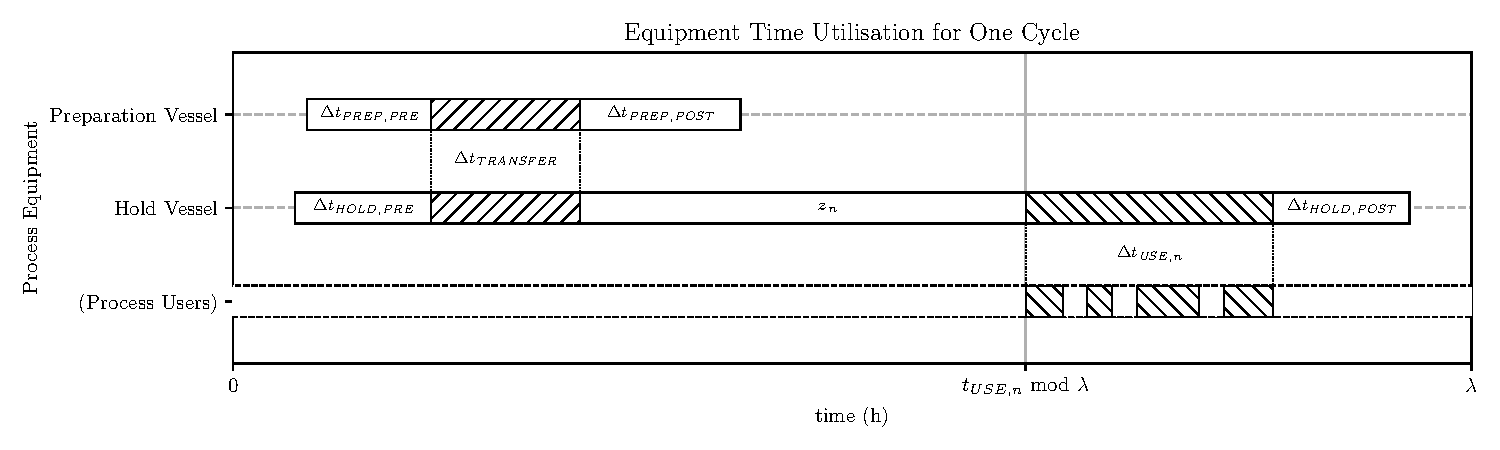
\includegraphics[width=\linewidth]{./figures/explanatory.pdf}
    \caption{Equipment time utilisation for a single buffer}
    \label{fig.explanatory}
\end{figure}
\begin{table}[h!]
    \centering
    \caption{Buffer data for random example}
    \label{tbl.buffer}
    \begin{tabular}{l | c | c | c}
        names & required volumes & use start times & use durations\\
        & $U_{n}$ (l) & $t_{\mathit{USE},n}^{*}$ (h) 
        & $\Delta t_{\mathit{USE},n}$
        (h)\\ \hline
        \text{Buffer \#1} & \SI{24427.13}{} & \SI{76.23}{} & \SI{20.56}{}\\
        \text{Buffer \#2} & \SI{5487.29}{} & \SI{0.21}{} & \SI{49.77}{}\\
        \text{Buffer \#3} & \SI{2588.36}{} & \SI{25.78}{} & \SI{24.56}{}\\
        \text{Buffer \#4} & \SI{7102.05}{} & \SI{46.79}{} & \SI{27.77}{}\\
        \text{Buffer \#5} & \SI{1020.87}{} & \SI{87.7}{} & \SI{36.58}{}\\
        \text{Buffer \#6} & \SI{19508.79}{} & \SI{35.52}{} & \SI{58.53}{}\\
        \text{Buffer \#7} & \SI{23073.55}{} & \SI{42.26}{} & \SI{39.71}{}\\
        \text{Buffer \#8} & \SI{25454.10}{} & \SI{48.38}{} & \SI{43.47}{}\\
        \text{Buffer \#9} & \SI{24088.67}{} & \SI{4.18}{} & \SI{55.41}{}\\
        \text{Buffer \#10} & \SI{3172.46}{} & \SI{48.31}{} & \SI{23.27}{}\\
        \text{Buffer \#11} & \SI{24752.71}{} & \SI{76.38}{} & \SI{45.80}{}\\
        \text{Buffer \#12} & \SI{13445.31}{} & \SI{73.93}{} & \SI{34.25}{}\\
    \end{tabular}
\end{table}

The buffer data will contain several parameters for each buffer to be prepared,
$n \in \mathcal{N}$.
A buffer data-set will contain entries for $N$ buffers:
\begin{equation}
    n \in \mathcal{N}; \quad \mathcal{N} = \left\{ 0, 1, 2, \ldots, n, \ldots,
    \left( N - 1 \right) \right\}
\end{equation}
\begin{equation}
    N = |\mathcal{N}|
\end{equation}
For each buffer, $n \in \mathcal{N}$, the data set will contain, at a minimum,
its required preparation volume (in litres), $U_{n}$.

If nothing was known about the scheduling of the production process, a simple
simulation could be carried out without scheduling.
Such a simulation would assume a fixed duration for all operations in the
preparation procedure and would require knowledge of the \emph{cycle time} (the
fixed duration from the start of one batch to the start of another batch) and
an additional parameter representing the maximum utilisation ratio of the
preparation vessels (see \hyperref[S.parameters]{Section \ref*{S.parameters}}).

For a complete model, with scheduling, we also need to know when each buffer
is first required by the process, and the duration for which it is required.

Sample buffer data are given in \hyperref[tbl.buffer]{Table \ref*{tbl.buffer}}.
\hyperref[fig.explanatory]{Figure \ref*{fig.explanatory}} gives an overview of
data and parameters related to scheduling, which are detailed in the remainder
of this section and in \hyperref[S.parameters]{Section \ref*{S.parameters}}.
The plot in \hyperref[fig.explanatory]{Figure \ref*{fig.explanatory}} is
termed an \emph{equipment time utilisation} plot; in this instance it just
shows the preparation and hold procedures for a single buffer.
This style of plot is covered in more detail in
\hyperref[C.results]{Chapter \ref*{C.results}}, where similar plots can be used
to visually display a working steady-state schedule for a feasible solution.

For each buffer, $n \in \mathcal{N}$, its (unnormalised) time of first use,
$t_{\mathit{USE},n}^{*}$, is the time when the process draws the first drop of
buffer from its hold vessel.
This time is relative to some batch datum, e.g.\ the start of the batch or the
start of downstream processing.
The choice of datum is unimportant once it is consistently used.
A campaign is a series of batches. 
The model deals with \emph{steady-state} processing (batches start with a fixed
cycle time and are assumed to be in the middle of a long campaign), so we are
interested in a single-cycle window.
Since we are looking at a single-cycle window at steady-state, the single-cycle
windows either side of it will be identical, and so on until we approach the
edges of the long campaign.
As a result, we want to normalise $t_{\mathit{USE},n}^{*}$ with respect to the
cycle time, $T$.
Accordingly, we define the (normalised) time of first use,
$t_{\mathit{USE},n}$:
\begin{equation}
    t_{\mathit{USE},n} = t_{\mathit{USE},n}^{*} \enspace \text{mod} \enspace 
    T \quad \forall n \in \mathcal{N}.
\end{equation}
Note that the random data generator used to produce the data in 
\hyperref[tbl.buffer]{Table \ref*{tbl.buffer}} produces values for 
$t_{\mathit{USE},n}^{*}$ that are already normalised, but for the real-world
examples discussed in \hyperref[C.results]{Chapter \ref*{C.results}}, 
$t_{\mathit{USE},n}^{*}$ may be unnormalised.

For each buffer, $n \in \mathcal{N}$, its duration of first use,
$\Delta t_{\mathit{USE},n}$, is the duration from when the process draws the
first drop of buffer from its hold vessel to when it finishes drawing the last
drop of buffer from the same vessel.
Note that a process may draw buffer discontinuously from a hold vessel, e.g.\ a
cleaning buffer may be drawn from its hold vessel for a few minutes at the end
of a chromatography procedure and may not be required again until near the end
of another chromatography procedure a day or two later, but may not be required
at all in the intervening period.
Note the use of the general convention that \emph{durations} are denoted by
$\Delta t$, whereas \emph{times} (relative to some datum) are denoted by $t$.
It is assumed that all times and durations are in hours.

For each buffer, $n \in \mathcal{N}$, $\Delta t_{\mathit{USE},n}$ must be
sufficiently less than the cycle time so that there is opportunity to
\emph{turn around} its hold vessel (i.e.\ sufficient time must exist after use
of the buffer to clean and sterilise the vessel, receive the subsequent batch
of the sane buffer and hold it for a sufficient duration before it is
required by the subsequent batch).

\section{Parameters}\label{S.parameters}

In addition to the buffer-specific and vessel-specific data detailed above,
some global parameters are required to specify the problem.
For the random example, these parameters are tabulated in
\hyperref[tbl.parameters]{Table \ref*{tbl.parameters}} and are described in
more detail hereafter.

\begin{table}[h!]
    \centering
    \caption{Global parameters for random example}
    \label{tbl.parameters}
    \begin{tabular}{l | l | r | c}
        symbol & short description & value & unit\\ \hline
        $T$ & process cycle time & 96.0 & h\\
        $\Delta t_{\mathit{PREP,PRE}}$ & prep pre duration & 12.0 & h\\
        $\Delta t_{\mathit{PREP,POST}}$ & prep post duration & 1.5 & h\\
        $\Delta t_{\mathit{TRANSFER}}$ & transfer duration & 2.0 & h\\
        $\Delta t_{\mathit{HOLD,PRE}}$ & hold pre duration & 8.0 & h\\
        $\Delta t_{\mathit{HOLD,POST}}$ & hold post duration & 1.5 & h\\
        $\Delta t_{\mathit{HOLD,MIN}}$ & minimum hold duration & 12.0 & h\\
        $\Delta t_{\mathit{HOLD,MAX}}$ & maximum hold duration & 60.0 & h\\
        $f_{\mathit{MINFILL}}$ & minimum fill ratio & 0.3 & --\\
        $f_{\mathit{UTIL}}$ & maximum utilisation ratio & 0.8 & --\\
    \end{tabular}
\end{table}

The first parameter specified is the cycle time, $T$.  We are concerned
with the steady-state operation of the process, so the cycle time can be
thought of as the duration from some fixed point in one batch to the same
fixed point in the subsequent batch.
The cycle time is typically some multiple of 24 hours.
This is for reasons of operability; it is easier for staff if a given task
occurs at the same time of the day for each batch.
Note that it is not our objective to seek to minimise the cycle time.
A well-designed facility should be bottlenecked at the production bioreactor,
so the cycle time is a function of the production process and not the buffer
preparation area.

In the model, the preparation and hold procedures are both broken into a number
of operations.
The durations of most of these operations are specified as global parameters.
It is unlikely that detailed timings will be available at the early stages of
design, so specifying some conservative global parameters provides a model that
is easy to comprehend and validate.
In reality, operations such as filling a vessel with water will scale with
buffer volume and operations such as cool-down of a vessel after steaming will
scale with vessel volume.
This degree of granularity could be added as a future model enhancement.

The following durations are specified as global parameters:

\begin{itemize}
\item
The parameter $\Delta t_{\mathit{PREP,PRE}}$ is the duration of all operations
in the preparation procedure prior to the transfer of buffer from the
preparation vessel to the hold vessel.  
This may include pressure testing, steam-in-place (SIP) and cool-down, although
these tasks are not always carried out on preparation vessels.
The period will include the charging of water for injection (WFI), the charging
of other liquids and/or solids, and time for mixing the buffer.
It may also include some time for sampling or testing and adjustment of the
buffer.
\item
The parameter $\Delta t_{\mathit{PREP,POST}}$ is the duration of all operations
in the preparation procedure that take place after the transfer of the buffer
to the buffer hold vessel is complete.
This is typically just comprised of the clean-in-place (CIP) of the vessel.
CIP involves a separate piece of equipment, the CIP skid, which circulates
cleaning fluids (detergents and/or acids, bases) through the vessel and some of
its attached pipework.
\item
The parameter $\Delta t_{\mathit{TRANSFER}}$ is the duration of the transfer
of buffer from the preparation vessel to the hold vessel, via a sterile filter.
Although this varies with the buffer volume, the relationship is not that
straightforward.
As buffer and vessel volumes increase, a change in pipe diameter or pump size
may be appropriate, giving large step changes to the transfer duration.
Accordingly, a conservative global parameter for transfer duration is
appropriate for early-stage design.
\item
The parameter $\Delta t_{\mathit{HOLD,PRE}}$ is the duration of all operations
in the hold procedure prior to the commencement of receipt of buffer from the
preparation vessel.
This typically includes pressure testing, SIP and cool-down.
\item
The parameter $\Delta t_{\mathit{HOLD,POST}}$ is the duration of all operations
in the hold procedure that take place after the last use of buffer by the
process is complete.
Like $\Delta t_{\mathit{PREP,POST}}$, this is primarily comprised of a CIP of
the respective vessel.
\item
Looking at \hyperref[fig.explanatory]{Figure \ref*{fig.explanatory}}, the one
symbol not yet mentioned is the buffer hold duration, $\boldsymbol{z}_{n}$.
Note that this is a decision variable, and not a parameter; it is discussed in
more detail in \hyperref[C.methodology]{Chapter \ref*{C.methodology}}.
The buffer hold duration is the duration that spans from the end of the
transfer into the buffer hold vessel until the start of the first use of the
buffer by the process.
As will be described in 
\hyperref[C.methodology]{Chapter \ref*{C.methodology}},
we place some bounds on this duration and express these bounds as a pair of
global parameters.
The parameter $\Delta t_{\mathit{HOLD,MIN}}$ defines the minimum allowable
duration of the buffer hold operation.
In practice, the operators of a plant do not want to schedule buffer
preparations so that the transfer is complete moments before the buffer is
required by the process, as any delays at this stage could impact production.
A value of $\Delta t_{\mathit{HOLD,MIN}}$, typically in the range of several
hours to one day, can be specified to ensure that buffers are prepared with
some flexibility to handle delays.
At the other end of the scale, buffers may expire and the global variable 
$\Delta t_{\mathit{HOLD,MAX}}$ is defined to set a maximum allowable hold
duration.
\item
When selecting a vessel, a minimum fill ratio, $f_{\mathit{MINFILL}}$ is
defined to ensure that a vessel isn't selected that is far too big for the
buffer being prepared. The rationale for this was discussed in
\hyperref[S.vesseldata]{Section \ref*{S.vesseldata}}.
\item
Finally, the utilisation ratio, $f_{\mathit{UTIL}}$, places an upper limit on
how busy a preparation vessel is allowed to be.
In the absence of detailed buffer scheduling information, this may represent an
`engineering factor' to account for unforeseeable scheduling clashes.
If detailed scheduling information is available, the ratio can be set to unity
to effectively remove its influence as a constraint, or the ratio could be
maintained at some value less than one to allow for overhead in the design.
\end{itemize}

\section{Data Sources}\label{S.sources}

\subsection{Random Data}\label{SS.randomdata}
The buffer data in \hyperref[tbl.buffer]{Table \ref*{tbl.buffer}} were randomly
generated.  
The parameters in \hyperref[tbl.parameters]{Table \ref*{tbl.parameters}} and
the vessel data in \hyperref[tbl.vessel]{Table \ref*{tbl.vessel}} are typical
figures based on the author's experience of designing and optimising
bioprocessing facilities.

A function was developed to generate random buffer data.
The function requires four inputs; the number of buffers required,
$\mathcal{N}$, the minimum duration ratio, $f_{\mathit{MINUSE}}$, the maximum
duration ratio, $f_{\mathit{MAXUSE}}$, and a `parameters' data set.
The function generates the required number of buffers, each with
$t_{\mathit{USE},n}^{*}$ uniformly distributed in the range
$0 < t_{\mathit{USE},n}^{*} < T$. Note that, for the random data, this means
that $t_{\mathit{USE},n}^{*} = t_{\mathit{USE},n}$, i.e.\ the random use
times are already normalised.
The use durations, $\Delta t_{\mathit{USE},n}$ are uniformly distributed and
depend on several parameters so that the model is feasible.  The feasible range
may be further scaled back using $f_{\mathit{MINUSE}}$ and
$f_{\mathit{MAXUSE}}$ to ensure values are credible, i.e.\
\begin{equation}
    f_{\mathit{MINUSE}} \times T < \Delta t_{\mathit{USE},n}
    < f_{\mathit{MAXUSE}} \times \Delta t_{\mathit{FEAS}}
\end{equation}
where
\begin{equation}
    \Delta t_{\mathit{FEAS}} = T - \left( 
    \Delta t_{\mathit{HOLD,PRE}}
    + \Delta t_{\mathit{TRANSFER}}
    + \Delta t_{\mathit{HOLD,MIN}}
    + \Delta t_{\mathit{HOLD,POST}} \right).
\end{equation}

These values are bound below by the minimum duration ratio times the cycle time

\subsection{Real-World Data}\label{SS.realdata}
Real-world data sets are based on mass balances and scheduling simulations
performed by the author for biopharmaceutical clients.
Since these processes are confidential, the data has been obfuscated in
several ways.
Firstly, the buffers are all given terse names, such as `Buffer \#1', and are
in no particular order.
Secondly, the buffer volumes may be scaled but only to a degree that does not
affect vessel selection.
Thirdly, the (normalised) duration parameters may all be scaled by a common
factor.
These changes serve to make the data unrecognisable but do not affect vessel
selection or scheduling (save for scaling the time axis).

Two real-world data sets are included as appendices to this report.



